\section{Paired Testing}
\begin{frame}
  \begin{center}
  {\bf Part II -- Paired Testing}
  \end{center}
\end{frame}

\subsection{Definitions}
\begin{frame}{Comparison of two means}{Dependent populations}

Suppose the following situation: a young researcher develops an optimization algorithm (A) {\bf for a given family of problems}, and wants to compare its convergence speed against a method that represents the state-of-the-art (B).
\bigskip

The researcher implements both methods and wants to determine whether the proposed one has a better average performance for problems of that particular family, which are represented by a given benchmark set.
\bigskip

The measurements are made under homogeneous conditions (same computer, same operational conditions, etc.) and the time is measured in a way that is not sensitive to other processes running in the system.
\end{frame}


\begin{frame}{Comparison of two means}{Dependent populations}
This problem has some important questions worth considering:
\bigskip

\begin{itemize}
  \item  What is the actual question of interest?
  \item What is the \textit{population} for which that question is relevant?
  \item What are the independent observations for that population?
  \item What are the relevant sample sizes for the experiment?
\end{itemize}
\bigskip

\begin{block}{}
  Consider carefully the difference between considering \emph{individual runs} as a population against \emph{individual problem instances} as a population. The important thing is to not mix both!
\end{block}
\end{frame}

\begin{frame}{Paired Experimental Design}

  The variability of results due to the different test problems is a strong source of spurious variation (noise) that can and must be controlled;\bigskip

  An elegant solution to eliminate the influence of this nuisance parameter is the \textit{pairing} of the measurements by problem:\bigskip

  \begin{itemize}
  \item Observations are considered in pairs (A, B) for each problem;
  \item Hypothesis testing is done on the sample of \textit{problem differences};
  \end{itemize}
\end{frame}

\begin{frame}{Paired Design}{Statistical Model}
Let $y_{Aj}$ and $y_{Bj}$ denote paired observations of average time for methods A and B, for each problem instance $j$. The \textit{paired difference} of an observation is simply $d_j = y_{Aj} - y_{Bj}$.
\bigskip

If we model our observations as an additive process:
\begin{equation*}
y_{ij} = \underbrace{\mu + \tau_i}_{\mu_i} + \beta_j + \varepsilon_{ij}
\end{equation*}
\noindent where $\mu$ is the grand mean, $\tau_i$ is the effect of the $i$-th method on the mean, $\beta_j$ is the effect of the $j$-th problem instance, and $\varepsilon_{ij}$ is the model residual, then:
\begin{equation*}
\begin{split}
d_j &= \mu + \tau_A + \beta_j + \varepsilon_{Aj} - (\mu + \tau_B + \beta_j + \varepsilon_{Bj})\\
d_j &= \cancelto{0}{\left(\mu +\beta_j - \mu - \beta_j\right)} + \tau_A-\tau_B + \varepsilon_{Aj}-\varepsilon_{Bj}\\
&=\mu_{D} + \varepsilon_j\\
\end{split}
\end{equation*}

\end{frame}

\begin{frame}{Paired Design}{Hypotheses}
The hypotheses of interest can now be defined in terms of $\mu_D$, e.g.:
\begin{equation*}\begin{cases}
H_0: \mu_D = 0\\
H_1: \mu_D \neq 0
\end{cases}\end{equation*}
\noindent which can now be treated as a test of hypotheses for a single sample: the population of interest is the differences in average times until convergence for the problems under investigation. The test statistic is given by:
\begin{equation*} T_0 = \frac{\bar{D}}{S_D/\sqrt{N}}\end{equation*}
\bigskip

which is distributed under the null hypothesis as a Student-t variable with $N-1$ degrees of freedom (where $N$ is the number of test problem instances in the experiment);
\end{frame}


\begin{frame}{Paired Design}{Considerations}
Some other important questions worth considering:
\medskip

\begin{itemize}
\item In this example the minimally interesting effect size $\delta^*$ must be expressed in terms of \textit{average time gains across problems} (not within individual instances);
\item The most important sample size to consider in this situation refers to the \textit{number of problem instances}, and not necessarily to the number of within-problems repeated measures;
\item The number of repetitions within each problem will have an impact on the uncertainty associated to each observation (that is, to each value of mean time to convergence for each algorithm on each problem), which will propagate down to the residual variance.
\end{itemize}
\end{frame}



\begin{frame}{Paired design}{Considerations}
Some other important questions worth considering:
\bigskip

\begin{itemize}
  \item Pairing removes the effects of controllable nuisance factors from the analysis.

  \item Strongly indicated in cases with {\bf strong correlations between samples} (e.g., heterogeneous experimental conditions).
\end{itemize}
\end{frame}

\subsection{Benchmark testing Example}

\begin{frame}{Paired Comparison Example}
Going back to our example, assume the following facts about the desired comparison:\bigskip

\begin{itemize}
\item The benchmark set is composed of seven problem instances ($N=7$);
\item The researcher is interested in finding differences in mean time to convergence greater than ten seconds ($\delta^*=10$) with a power of at least $(1-\beta)=0.8$, using a significance level $\alpha=0.05$;
\item The researcher performs $n=30$ repeated runs\footnote[1]{\tiny Not that this number is necessarily good, but it is generally an easy alternative if you don't want to keep justifying your choices to less statistically-savvy reviewers.} of each algorithm in each problem, from random initial conditions.
\end{itemize}

\end{frame}




\begin{frame}[fragile]{Executing the Paired Analysis}
  {Step 1: load and precondition the data}
{\smaller{\smaller
\begin{verbatim}
> # Read data
> data <- read.table("benchmark.csv",
+                    header=T)

# "Problem" is a categorical variable, not a continuous one
> data$Problem <- as.factor(data$Problem)

# Summarize within-problem observations by mean
> aggdata <- aggregate(Time ~ Problem:Algorithm,
+                      data = data,
+                      FUN  = mean)
> summary(aggdata)
 Problem Algorithm      Time
 1:2     A:7       Min.   : 37.63
 2:2     B:7       1st Qu.:109.45
 3:2               Median :178.73
 4:2               Mean   :175.48
 5:2               3rd Qu.:245.25
 6:2               Max.   :296.79
 7:2
\end{verbatim}}}
\end{frame}



\begin{frame}[fragile]{Executing the Paired Analysis}{Step 2: analysis}
  {\smaller{\smaller
\begin{verbatim}
> # Perform paired t-test
> t.test(Time ~ Algorithm,
+        paired = TRUE,
+        data   = aggdata)

Paired t-test
data:  Time by Algorithm
t = -9.1585, df = 6, p-value = 9.54e-05
alternative hypothesis: true difference in means is not equal to 0
95 percent confidence interval:
 -21.85862 -12.64118
sample estimates:
mean of the differences
               -17.2499
\end{verbatim}}}
\end{frame}



%=====

\begin{frame}[fragile]
{Executing the Paired Analysis}
{Alternatively, we could have done:}

{\smaller{\smaller
\begin{verbatim}
> difTimes <- aggdata$Time[1:7] - aggdata$Time[8:14])
> t.test(difTimes)


One Sample t-test
data:  difTimes
t = -9.1585, df = 6, p-value = 9.54e-05
alternative hypothesis: true mean is not equal to 0
95 percent confidence interval:
 -21.85862 -12.64118
sample estimates:
mean of x
 -17.2499
\end{verbatim}}}
\bigskip

{\bf Check your understanding:} Why is the paired test on two samples equivalent to the one sample test on the difference vector of the samples?
\end{frame}

\begin{frame}[fragile]{Verifying the Assumptions}
  \begin{columns}
    \column{0.6\textwidth}
{\smaller{\smaller
\begin{verbatim}
> shapiro.test(difTimes)

Shapiro-Wilk normality test
data:  difTimes
W = 0.8387, p-value = 0.09655

# Redo test without outlier
> indx <- which(difTimes == max(difTimes))
> t.test(difTimes[-indx])$p.value
[1] 6.179743e-06
> t.test(difTimes[-indx])$conf.int
[1] -21.41856 -16.48037
\end{verbatim}}}
\column{0.4\textwidth}
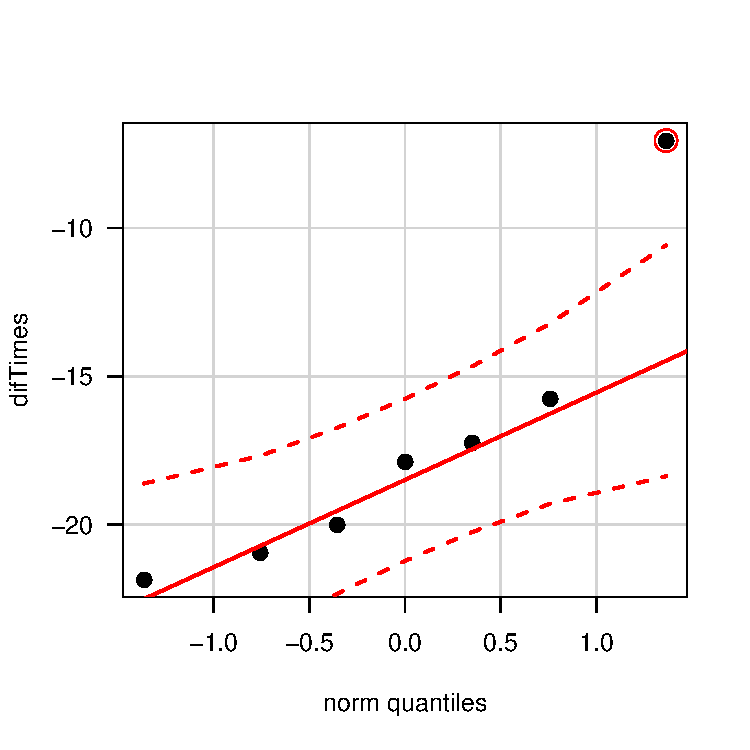
\includegraphics[width=\textwidth]{../img/soltimesqq.pdf}
\end{columns}
\end{frame}



%=====

\begin{frame}[fragile]{Why is Pairing Important?}
What happens if we fail to consider the problem effects?
{\smaller{\smaller
\begin{verbatim}
> t.test(Time ~ Algorithm, data = aggdata)

Welch Two Sample t-test
data:  Time by Algorithm
t = -0.3609, df = 11.993, p-value = 0.7245
alternative hypothesis: true difference in means is not equal to 0
95 percent confidence interval:
 -121.40320   86.90341
sample estimates:
mean in group A mean in group B
       166.8527        184.1026
\end{verbatim}}}
\bigskip

Failure to consider inter-unit variability can result in the masking of relevant effects by the nuisance factor.
\bigskip

Similarly, failure in recognizing the dependence structure of within-unit measurements yields tests with artificially inflated degrees of freedom, which results in the inflation of the effective value of $\alpha$.
\end{frame}

%=====
%
% \begin{ftstf}
% {Comparison of two means}
% {Paired design}
% Paired designs can require smaller sample sizes for equivalent power in cases where the between-units (in our example, the between-problems) variation is relatively high;
% \vhalf
% More specifically, if the within-level variation is given by $\sigma_\epsilon$ and the between-units variation is $\sigma_u$, we have that, for large enough $N$\\(e.g., $N\geq 10$),
% \beqs
% \frac{N_{\mbox{\tiny unpaired}}}{N_{\mbox{\tiny paired}}}\approx\sqrt{2\left[\left(\frac{\sigma_u}{\sigma_\epsilon}\right)^2+1\right]}
% \eqs
% \vhalf
% Failure to consider inter-unit variability can result in the masking of relevant effects by the nuisance factor.
% \vhalf
% Similarly, failure in recognizing the dependence structure of within-unit measurements yields tests with artificially inflated degrees of freedom, which results in the inflation of the effective value of $\alpha$.
% \end{ftstf}

%% My slide: A few more examples of paired testing.
